\documentclass{amsart}
\usepackage[british]{babel}
\usepackage{url}
\usepackage{hyperref}
\usepackage{xcolor}
\usepackage{enumerate}
\usepackage{tikz}
\usepackage{pgfplots}
\usepackage{draftwatermark}
\SetWatermarkText{\textsc{Draft -- Not for Circulation}}
\SetWatermarkScale{2}
\definecolor{edblue}{RGB}{0,0,153}
\hypersetup{
  pdftitle={\@title{}},
  colorlinks=true,
  linkcolor=edblue,anchorcolor=edblue,citecolor=edblue,filecolor=edblue,urlcolor=edblue
}%
\usepackage{geometry}
\geometry{a4paper,textwidth=5.5in,textheight=8.5in,marginparsep=7pt,marginparwidth=.6in}
\usepackage{graphicx}
\usepackage{wrapfig}
\RequirePackage[hyperref=true,
  url=true,
  isbn=true,
  backref=false,
  bibstyle=ieee,
  citestyle=authoryear-icomp,
  maxcitenames=3,
  maxbibnames=100,
  backend=biber,
  block=none]{biblatex}
\addbibresource{literature.bib}
\title{Report on new equipment for community broadband}
\author{P. Buneman \and M. Fourman \and W. Waites}
\begin{document}
\begin{center}
  {\Huge\textbf{\color{red}DRAFT -- NOT FOR CIRCULATION}}
\end{center}
\maketitle
\tableofcontents
\section{Summary}
The Demonstrating Digital Programme of Scottish Government provided a small grant to the
University of Edinburgh to test wireless equipment that may be useful in the
deployment of rural community broadband.  Although most community
networks are currently limited not by the speed of their wireless
links, but by the available bandwidth, it is to be hoped that this
will be improved with the current....

A manufacturer of low-cost wireless distribution hardware has recently
released some low cost equipment operating in the 24GHz and 5GHz
spectrum.  If it lives up to its specifications, it offers an order of
magnitude increase in the capacity of current point-to-point links
over existing technology that operates in the spectra that are
available to com
munites.  In addition we tested laser (free-space
optics) equipment operating in an urban environment but also serving
rural communities.

To summarise our findings.
\begin{itemize}
\item The 24 GHz equipment could prove useful over relatively short
distances (up to 8 km) if licencing permitted use at the power for
which it is designed.

\item Given the current power limits and available bands in the 
5GHz range, the 5GHz equipment probably provides only a minor
improvement on what could be achieved by using two or three parallel
links using lower cost equipment in different bands.  There is, of
course, a simplicity/redundancy trade-off. Moreover the 5GHz equipment
was sensitive to tidal fading and occasionally failed completely (perhaps
due to the presence of marine radar)

\item The free-space optics equipment performs, as expected, well over
  distances of a few hundred metres, but will not be useful for longer
  links in a rural (Scottish)
  environment\footnote{Figure~\ref{fig-cloudy} shows the ``free-space''
    conditions on one of the shortest Tegola links.  The camera is at one relay
    and the next relay is about 2km away on the hill in the
    background.}. The equipment is expensive, and beyond the reach of
  a small community project, though we might have   been able to
  reduce the cost by using an alternative vendor.
\end{itemize}

The main obstacle to using the 5 and 24 GHz equipment is licencing.
Under current regulations the 24GHz is effectively useless, and the 5GHz
equipment would be much more useful if (a)  the power limits were to
be raised and (b) Ofcom were to publish their database of licences in
the C band.

\begin{figure}
  \begin{center}
    \includegraphics[width=0.49\textwidth]{sgritheall-clear.jpg}%
    \hfill%
    \includegraphics[width=0.49\textwidth]{sgritheall-cloudy.jpg}
  \end{center}
\label{fig-cloudy}
\caption{Scotch mist}
\end{figure}
\section{Introduction}\label{introduction}
Many community broadband projects require a long-range wireless link
for their connection to the Internet. The equipment of choice is
currently based on wifi operating in the unlicensed 2.4 or 5GHz
spectra. This is cheap: the equipment for a long-distance
point-to-point link costs under \pounds 400 and can provide
bi-directional throughput of about 50Mb/s. While this provides an
improvement for the many rural communities that are served by long
copper telephone lines, 50Mb/s is no longer adequate for a community
of, say, 50 residences. Technically, there is no problem in getting
more bandwidth in one of the licenced spectra, but the equipment is
more expensive and the additional cost of the licence makes this
option unaffordable for small communities.

Recently some new equipment operating at 24GHz has come on the market
from Ubiquiti\footnote{\href{http://www.ubnt.com/airfiber}{\url{http://www.ubnt.com/airfiber}}}.
This is advertised as offering 1.4Gb/s at up to 13km. Although not as
cheap (a point-to-point link costs about \pounds 3,000) it might present
an opportunity for some rural communities to upgrade their service to
be competitive with the current fibre based offerings in the UK,
assuming they can find an internet connection with that bandwidth. A
5GHz variant is also produced by Ubiquiti claiming comparable speeds
at upwards of 50km.

With this in mind, the Scottish Government's Demonstrating
Digital programme provided the University of Edinburgh with funds to
test this equipment ``in the wild''. Of course, there is ample evidence
that the equipment works, but most of the evidence we have is
from installations in urban areas over short distances. How will
it perform over longer distances in West Highland weather? And what
are the practical problems faced by communities who want to install it?

At the request of the Scottish Government we also evaluated an
unrelated technology for use in urban areas -- free-space optics. This
means signalling by laser through the air instead of through
fibre-optic cabling. The main question here was, since these devices
operate in the visible spectrum, how well do they operate in reduced
visibility conditions? Do they operate \emph{well enough} for use in
this climate over short distances. Again it is a question of cost. The
equipment is expensive (some \pounds 8-15k per link) and requires
careful mounting and alignment, but compared to the civil engineering
cost of running fibre in urban areas, or leasing it, it may be worth
it.

\clearpage
\section{24GHz experiments}\label{ghz-experiments}

\subsection{Background}\label{background}

Before going into an account of the the project, let us look at some of
the pros and cons of using this equipment and what is already
known about wireless transmission in the 24 GHz spectrum. We have
already noted that the equipment is affordable. The advertised
throughput of 1.4Gb/s presumably means 700Mb/s in each direction, but
that would provide a satisfactory connection for a hundred or
so residences. Moreover, transmission in this frequency is much
less likely to be affected by tidal reflection (a significant problem
in the Highlands and Islands)

There are some significant drawbacks, though.

\begin{itemize}
\item
  In the UK, the 24.050--24.250GHz band is partitioned into two
  sub-bands, although the 24GHz spectrum is unlicenced the power 
  limits are such that it is unlikely that this equipment would be 
  effective over the distances we have in mind. We obtained a 
  ``non-operational'' licence from Ofcom in order to test the
  equipment  at the advertised power.
\item
  Several of the links used by Tegola and related projects are longer 
  than 13km
\item
  Transmission in higher frequencies is adversely affected by high 
  humidity and high temperatures. Scotland benefits from only one of 
  these.
\item
  The Ubiquiti equipment uses substantially more power than their 5GHz 
  offerings -- about 40W. This would make it unsuitable for solar and 
  wind-powered relays.
\end{itemize}

Our initial plan was to test the equipment on existing Tegola
relays one is a 6.5km link; the second 15.5km. Although the latter is
over the advertised range, even a substantial fraction of the
advertised throughput would be useful.

The following is a roughly chronological account of the project.
The initial installation was done during a period of very high winds
in early January 2014.

\subsection{Initial configuration and testing}
\label{december-2013-initial-configuration-and-testing}

\begin{wrapfigure}{r}{0.3\textwidth}
\includegraphics[width=0.3\textwidth]{radio-in-corridor}
\end{wrapfigure}
We ordered and received one pair of radios. Before deploying them
we thought it would be a good idea to check that they were working
and test them in ideal situation -- our office corridor. One thing
we immediately noticed was how critical alignment is. Even over
a distance of 35m, the performance fell of dramatically if the
antennae were slightly out of alignment. It's a very good idea to
configure equipment before deploying it, but to do this we had to turn
off sychronisation which relies on GPS and doesn't work indoors.

\subsection{Strengthening the masts}
\label{december-2013-january-2014-strengthening-the-relays}

Our basic relay construction (see the
\href{http://www.tegola.org.uk/howto/relay-construction.html}{relevant
  howto on the Tegola web site}) uses aluminium pegs to anchor the
diagonal braces to the ground. Both sites were on terrain that
consisted of bedrock covered by peat of varying depth. Although we
have never had a problem with the pegs shifting, peat is a bit
jelly-like, and the structures can wobble through a cm or two. The
alignment of 24GHz is much more critical than for the lower bandwidths
of 2.4 and 5.8GHz, so we replaced the pegs with epoxy bolts into the
bedrock.
\begin{figure}[h]
\includegraphics[width=0.4\textwidth]{corran-peg}
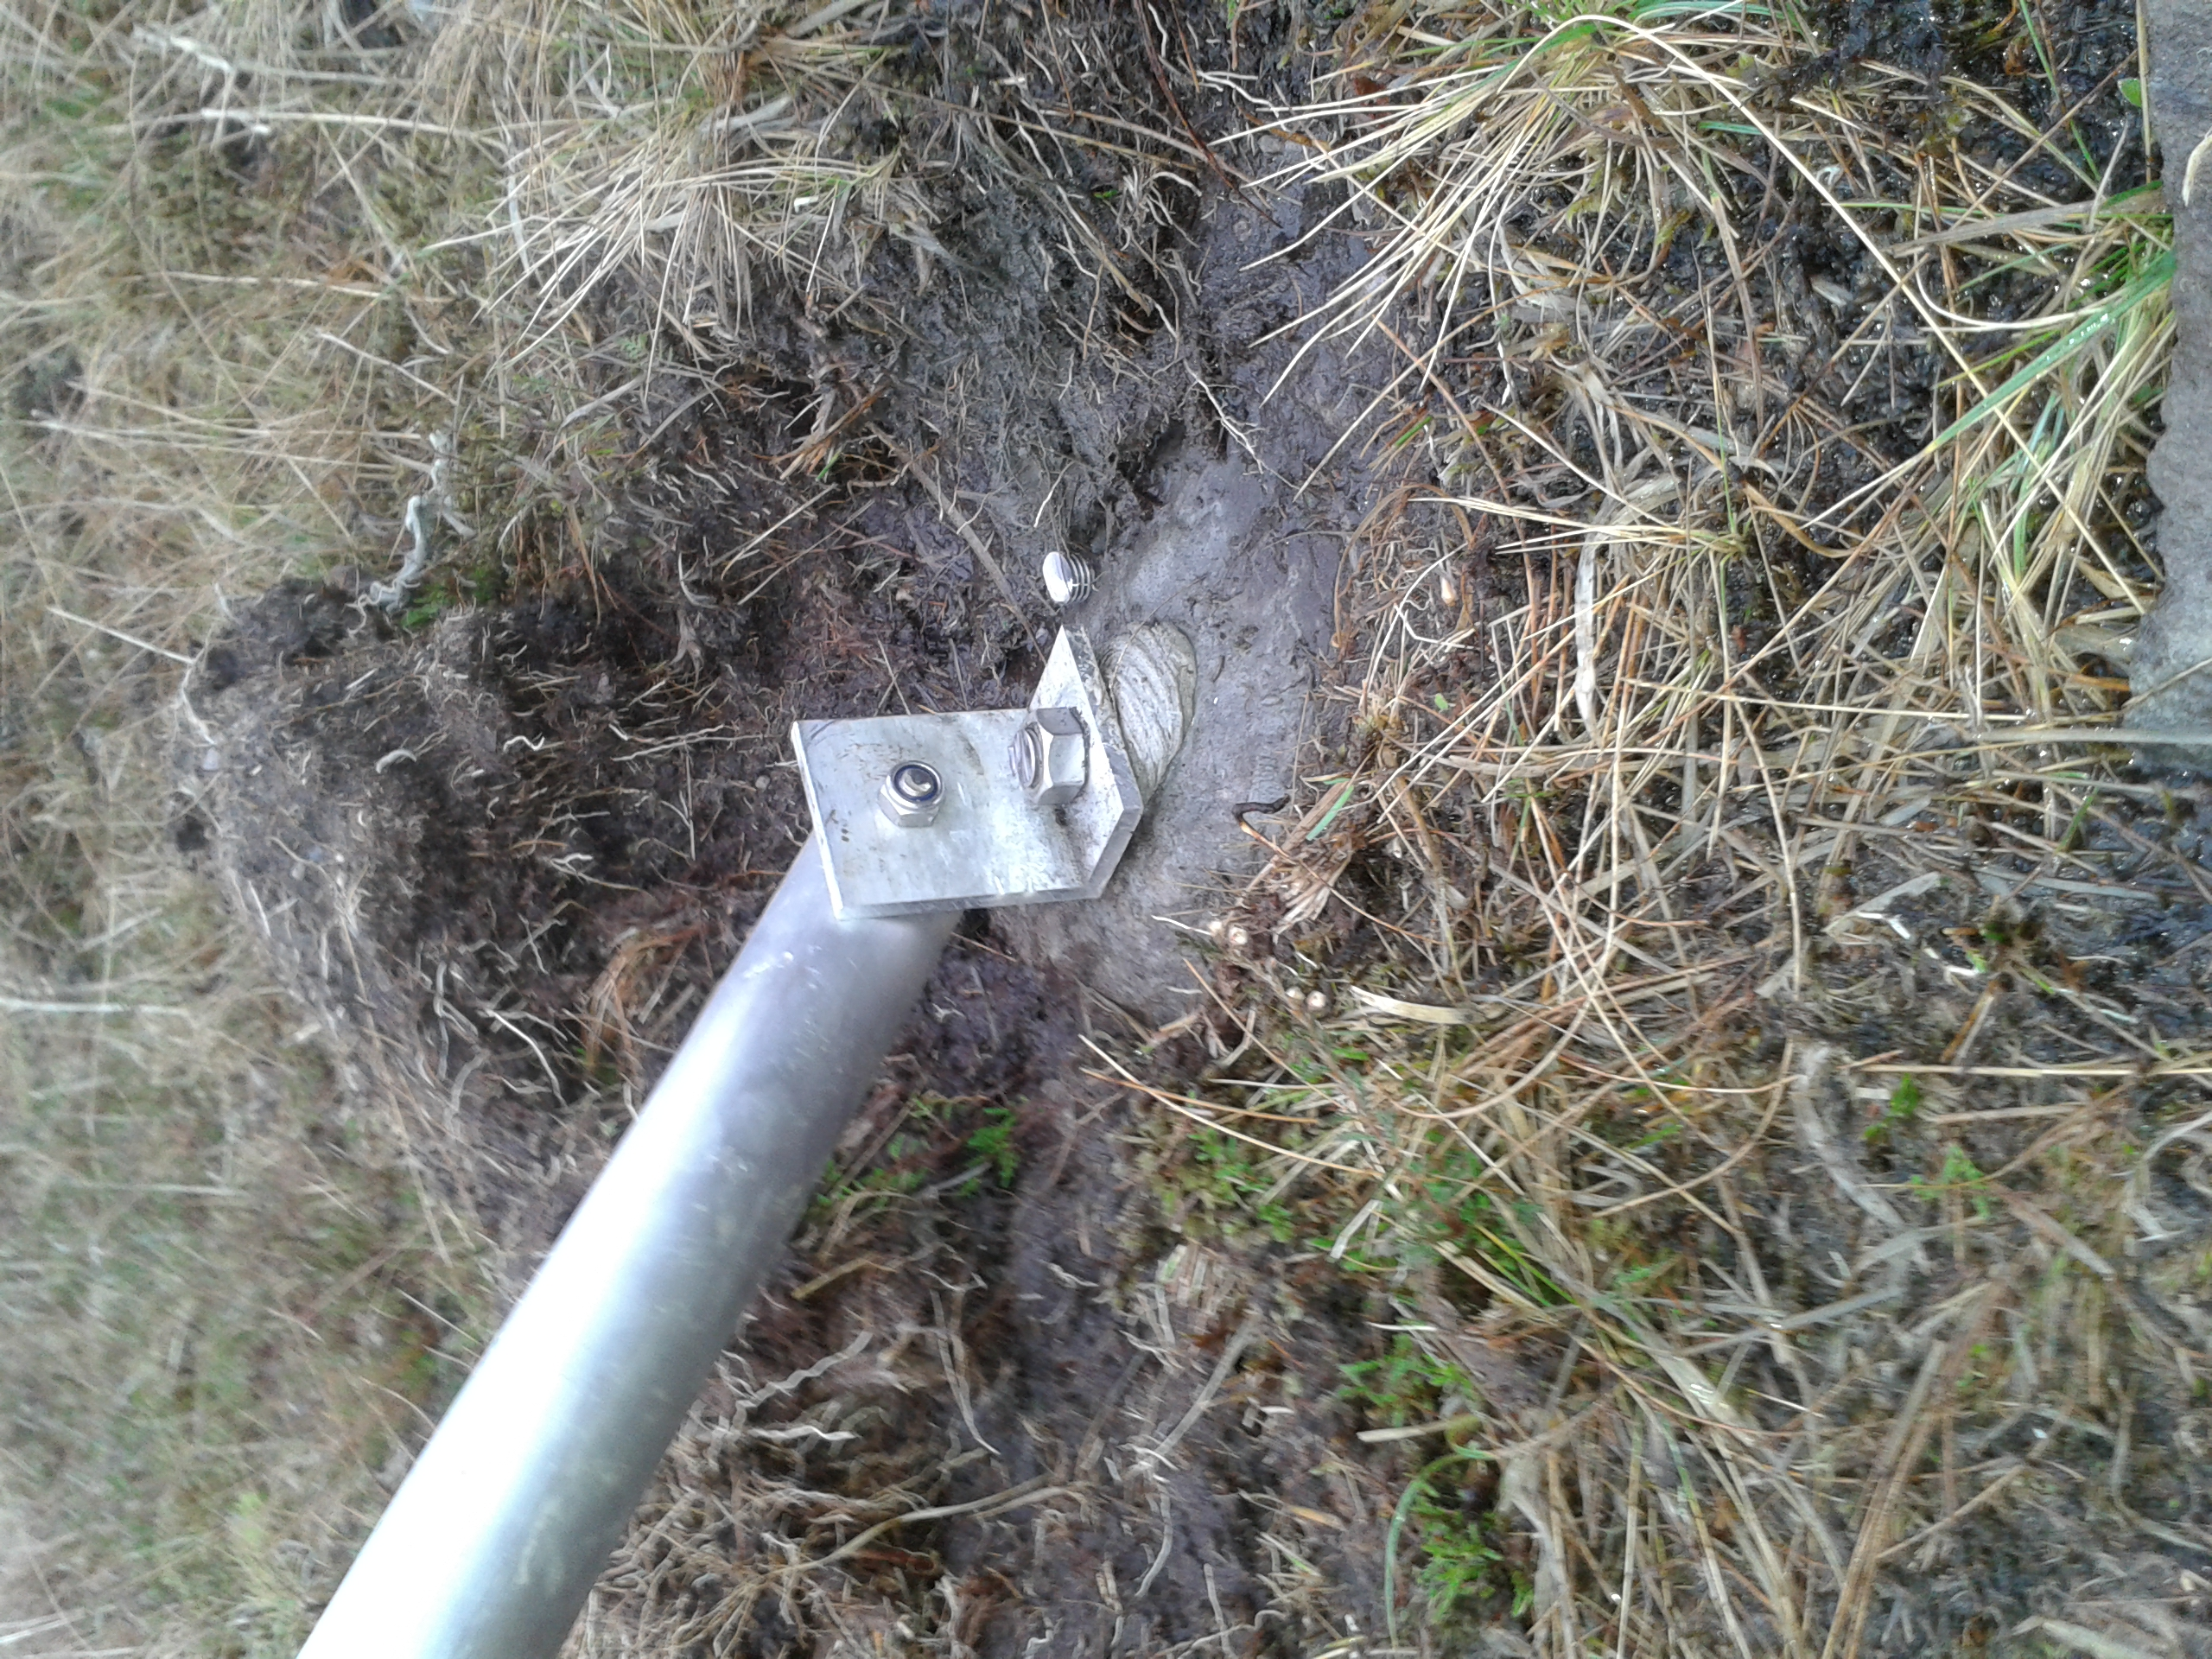
\includegraphics[width=0.4\textwidth]{corran-epoxy}
\caption{Pegged anchors (left) and epoxied anchors (right).}
\end{figure}

We also strengthened both relays. For example, at one of our relays we
added an extra horizontal bar.

\begin{figure}[h]
\includegraphics[width=0.4\textwidth]{corran-before-from-behind}
\includegraphics[width=0.4\textwidth]{corran-after-from-behind}
\caption{Corran mast before (left) and after (right)}
\end{figure}

\subsection{Installation and alignment}
\label{january-2014.-installation-and-alignment}

The radios are reasonably light (under 10kg) but awkward to carry up
hills. We used an old backpack frame that 30 years ago had been used
for carrying batteries up to community TV relays. The radios come with
a mounting frame that is first attached to the structure. The radio is
then ``slotted'' into the mounting frame. This arrangement makes it
quite easy to install the whole assembly when working from a ladder.

The antenna can be aligned through elevation and azimuth
adjustment screws. Unfortunately there is a great deal of backlash in
these screws, and they are almost useless if you are working in high
winds. If the clamping bolts are loose, the antenna is blown around
through the considerable travel allowed by the adjustment screws. The
signal strength read-out is at the bottom of the antenna, and if
the alignment is being done from a ladder, you almost certainly
need someone below (with a hard hat) to squint up and call out
the figures.

The installation instructions recommend an alternating process in which
one end of the link is adjusted then the other, and so
on. Unfortunately we were unable to complete this process before
the weather closed in and our workforce departed. However, the
alignment is good enough that we can start taking some measurements.
The initial indications are that the link will work reasonably well
over a distance of 6.5km.

\subsection{Performance}\label{performance}

\clearpage

\section{Free-space Optics}
\label{sec:fso}


%%% Local Variables:
%%% mode: latex
%%% TeX-master: "scotgov-report"
%%% End:

\clearpage
\printbibliography
\end{document}

%%% Local Variables:
%%% mode: latex
%%% TeX-master: t
%%% reftex-default-bibliography: ("literature.bib")
%%% zotero-collection: #("28" 0 2 (name "Papers/Scotgov Report"))
%%% End:
